% Use only LaTeX2e, calling the article.cls class and 12-point type.

\documentclass[12pt]{article}

% Users of the {thebibliography} environment or BibTeX should use the
% scicite.sty package, downloadable from *Science* at
% www.sciencemag.org/about/authors/prep/TeX_help/ .
% This package should properly format in-text
% reference calls and reference-list numbers.

%\usepackage{scicite}

% Use times if you have the font installed; otherwise, comment out the
% following line.
\setlength{\parindent}{2em}
\usepackage{indentfirst}
\usepackage{graphicx} % Required for including images
\usepackage{subfig}
\graphicspath{{figures/}} % Location of the graphics files
\usepackage{times}
\usepackage{xeCJK} %调用 xeCJK 宏包
\setCJKmainfont{STSong} %设置 CJK 主字体为 SimSun (宋体)
%\setCJKmainfont[BoldFont=STZhongsong]{STSong}
\setCJKsansfont[BoldFont=STHeiti]{STXihei}
\setCJKmonofont{STFangsong}
% The preamble here sets up a lot of new/revised commands and
% environments.  It's annoying, but please do *not* try to strip these
% out into a separate .sty file (which could lead to the loss of some
% information when we convert the file to other formats).  Instead, keep
% them in the preamble of your main LaTeX source file.


% The following parameters seem to provide a reasonable page setup.
\graphicspath{{figures/}}
\topmargin 0.0cm
\oddsidemargin 0.2cm
\textwidth 16cm 
\textheight 21cm
\footskip 1.0cm


%The next command sets up an environment for the abstract to your paper.

\newenvironment{sciabstract}{%
\begin{quote} \bf}
{\end{quote}}


% If your reference list includes text notes as well as references,
% include the following line; otherwise, comment it out.

%\renewcommand\refname{References and Notes}

% The following lines set up an environment for the last note in the
% reference list, which commonly includes acknowledgments of funding,
% help, etc.  It's intended for users of BibTeX or the {thebibliography}
% environment.  Users who are hand-coding their references at the end
% using a list environment such as {enumerate} can simply add another
% item at the end, and it will be numbered automatically.

\newcounter{lastnote}
\newenvironment{scilastnote}{%
\setcounter{lastnote}{\value{enumiv}}%
\addtocounter{lastnote}{+1}%
\begin{list}%
{\arabic{lastnote}.}
{\setlength{\leftmargin}{.22in}}
{\setlength{\labelsep}{.5em}}}
{\end{list}}


\usepackage{biblatex}	% Use biblatex
\addbibresource{scibib.bib}	

% Include your paper's title here

\title{使用CGAN对图形验证码的优化\\ \normalsize{(基于FashionMNIST数据集)}} 


% Place the author information here.  Please hand-code the contact
% information and notecalls; do *not* use \footnote commands.  Let the
% author contact information appear immediately below the author names
% as shown.  We would also prefer that you don't change the type-size
% settings shown here.

\author
{张知行 \\
\\
\normalsize{清华大学 \ 材料学院}\\
%\normalsize{An Unknown Address, Wherever, ST 00000, USA}\\
%\normalsize{$^{2}$Another Unknown Address, Palookaville, ST 99999, USA}\\
%\\
%\normalsize{$^\ast$To whom correspondence should be addressed; E-mail:  jsmith@wherever.edu.}
}

% Include the date command, but leave its argument blank.

\date{}



%%%%%%%%%%%%%%%%% END OF PREAMBLE %%%%%%%%%%%%%%%%



\begin{document} 

% Double-space the manuscript.

\baselineskip24pt

% Make the title.

\maketitle 



% Place your abstract within the special {sciabstract} environment.

\begin{sciabstract}
    传统的验证码主要由数字或字符构成,在图像识别技术相当成熟的时代,已经难以满足安全性的要求。因此,使用一种对机器较为难以识别但是肉眼可以轻易辨别的验证手段十分必要。为了克服传统验证码的缺陷,我们创新地决定使用衣饰用品图片作为验证码。在此基础上,我们设计了一种可以产生种类明确,易于肉眼区分的图片的方式来适应网络应用的发展。

  FashionMNIST\supercite{DBLP}是一个由$28\times 28$的灰度图片构成的衣饰用品数据集,具有相比于传统的MNIST更高的辨别模型训练难度。我们在FashionMNIST数据集上使用CGAN进行了模型构建与训练,并将生成的图片与已经证明得到较好验证效果的生成模型PGGAN\supercite{DBLP:journals/corr/abs-1710-10196}生成的图片进行对比,说明了我们的模型存在一定的优势并可以更好地应用于当前的验证码图片生成当中。

\end{sciabstract}


\section*{Introduction}

  互联网应用的发展十分迅速,几乎所有的服务商都提供互联网服务。验证码是一种区分用户是计算机还是人的公共全自动程序,可以用来有效防止恶意破解密码、刷票、论坛灌水等行为,是一种为了保证网络应用服务手段的有效方式。但是目前大部分的验证码都是使用数字或者字母验证码的阶段。对于数字和字母验证码,目前已经有了有效的使用技术手段破解的方式\supercite{10.1007}。传统的验证码在很大程度上已经难以实现区分人类和机器的目标。因此,使用一种对机器较为难以识别但是肉眼可以轻易辨别的验证手段十分必要。同时,使用现有的数据集来制作的验证手段十分容易通过算法进行识别。因此为了适应网络应用的发展,我们需要大量种类明确,易于肉眼区分但是机器难以分辨的图片。


 GAN\supercite{NIPS2014_5423}(Generative Adversarial Networks)是GoodFellow在2014年的论文中提出的一种思想,要求Generator学习将一个已知的高斯分布映射到更高维的空间中去拟合真实图像的分布。简单来说,GAN是一种将生成模型与判别模型进行结合来实现更好的生成的方式。

%  GAN具有很好地应用前景,从目前的文献来看,GAN 在图像上的应用主要是向图像修改方向发展。涉及的图像修改方向主要包括:单图像超分辨率、交互式图像生成、图像编辑、图像到图像的翻译等。

 但是朴素的GAN存在模型过于自由不可控的缺陷。同时,朴素的GAN中生成的结果并不含有标签,无法直接用于我们需求的场景当中。因此我们选取CGAN\supercite{DBLP:journals/corr/MirzaO14}(Conditional Generative Adversarial Nets)作为我们模型的基础。CGAN的简要结构如图\ref{cgan}所示。

\begin{center}\vspace{1cm}
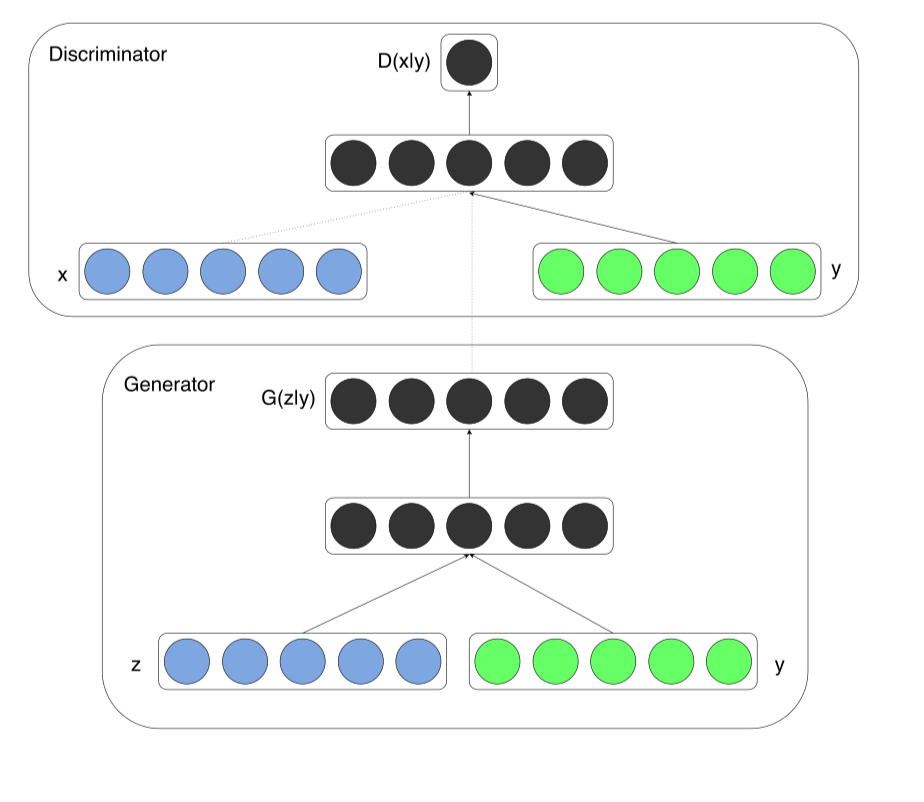
\includegraphics[width=0.6\linewidth]{CGAN.png}
\captionof{figure}{\color{Green} CGAN基本结构\supercite{DBLP:journals/corr/MirzaO14}}
\label{cgan}
\end{center}\vspace{1cm}

 在此基础上,我们设计了相应的算法并进行了一系列的参数调整来实现尽可能最优的结果。我们对最后生成的结果与渐进式的模型中得到的结果进行了比较,验证了我们的模型的良好表现并说明了我们的方式的良好的应用前景。

\section*{Main Objectives}

\begin{enumerate}
\item 在CGAN模型的基础上设计一个适用于FashionMNIST数据集的算法并实现。
\item 通过大量的实验对设计的模型进行参数调优。
\item 对PGGAN模型中源码进行修改并在相同数据集下进行训练得到最终输出结果。
\item 对两种模型下的表现进行分析并验证我们模型在验证码生成情形下的优势。
\item 使用图像识别程序对我们生成的验证图片和使用现有数据集生成的图片进行判断,验证我们生成的图片的优势性。
\end{enumerate}


\section*{Methods \& Experiments}

  基于\cite{DBLP:journals/corr/MirzaO14}中的设计思想,我们设计了图\ref{demo}中的网络作为我们的基本模型并在此基础上进行训练与模型调整。我们使用的训练机器为配置了4核心Intel(R) Core(TM) i5-7500 CPU @ 3.40GHz,24G RAM,GTX 1080Ti的Ubuntu16.04极客云服务器,我们的代码编写环境为Python=3.6。
\begin{center}\vspace{1cm}
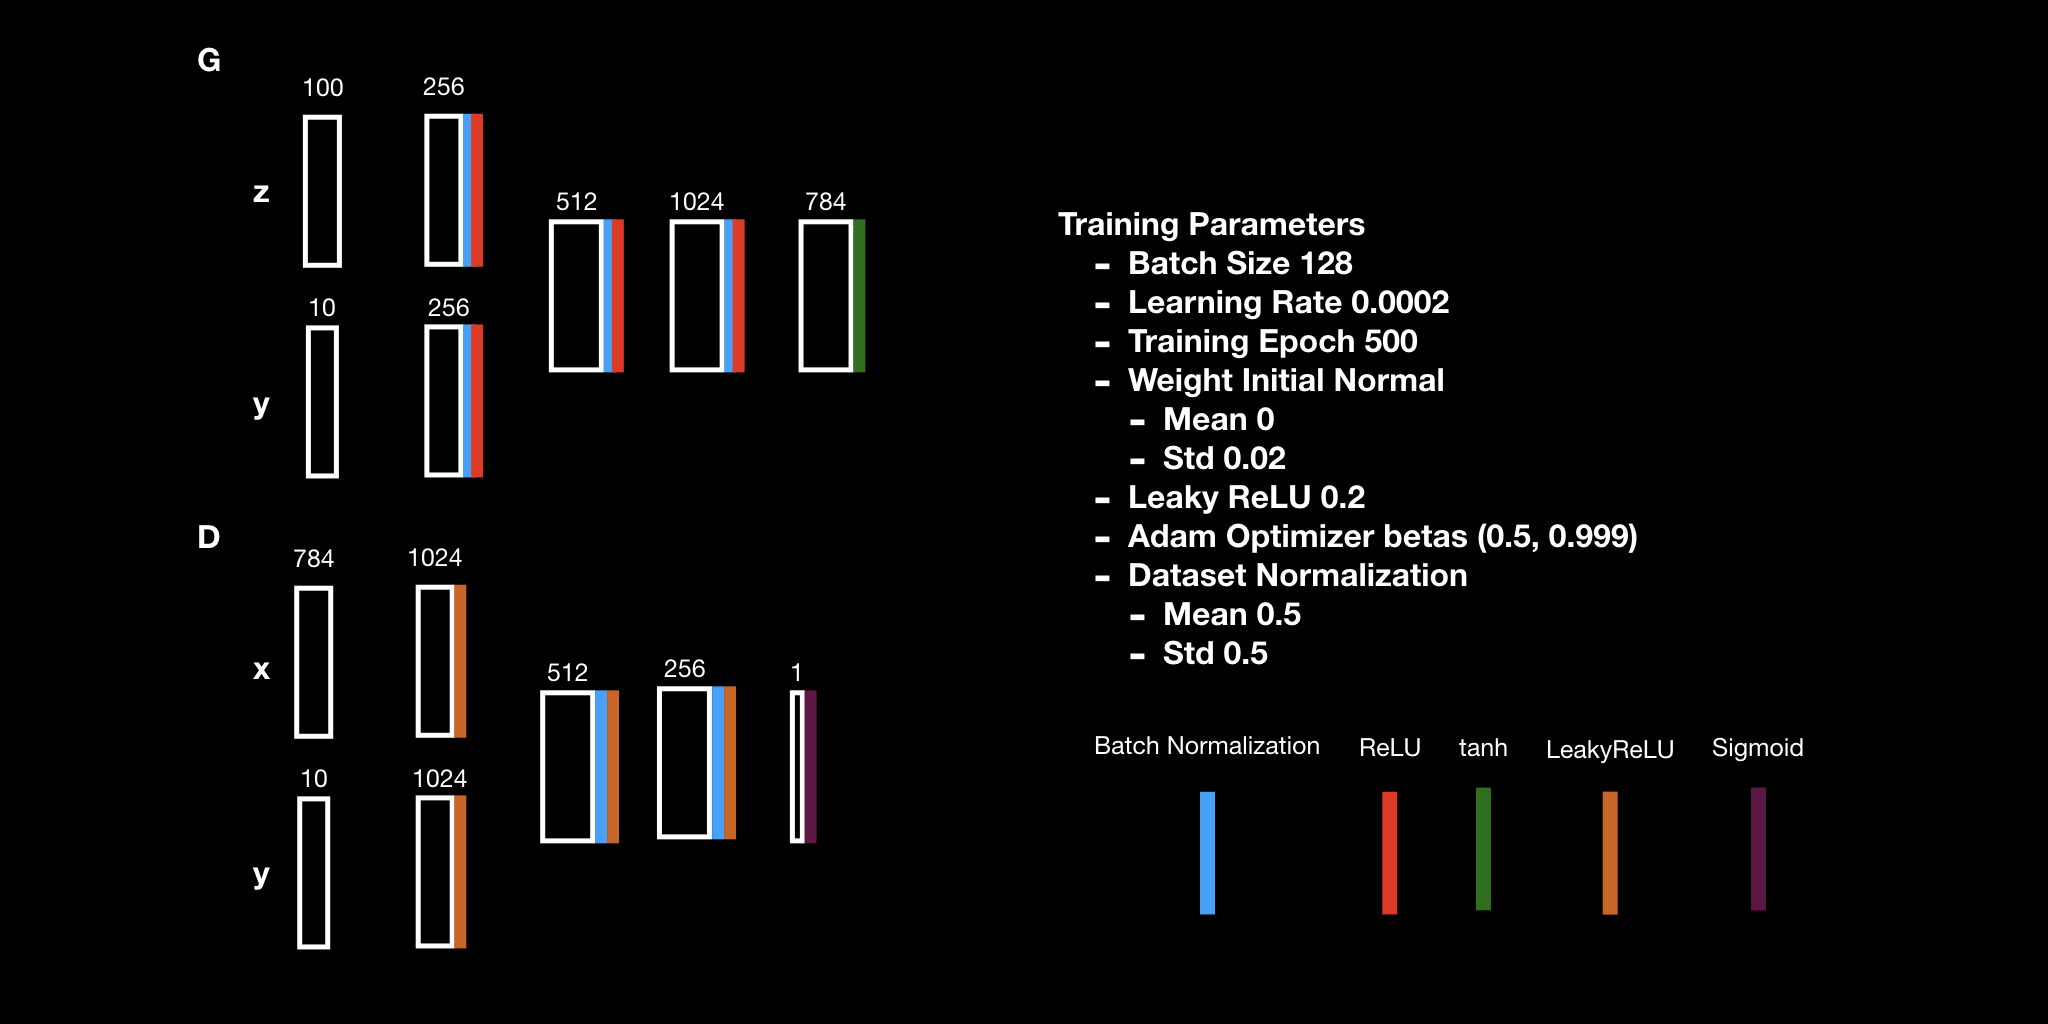
\includegraphics[width=1.0\linewidth]{demo.jpeg}
\captionof{figure}{\color{Green} Framework}
\label{demo}
\end{center}\vspace{1cm}


\subsection*{Experiments \& Parameters Modification}
%-----------------------------------------------
\begin{enumerate}
	\item 基本思路:根据不同情况采取不同的策略灵活调整学习率。
	\item 基本策略:我们使用BCELoss作为损失函数,以相隔一定间距的损失函数值是否下降为标准,判断损失函数是否已经接近要达到的极小值;已经接近的时候乘一个折合系数。
	\item 改进:根据具体在数据集上运行的表现,在不同的迭代次数区间选取不同的判断间距和折合系数。
	\item 效果:经过多次调整和尝试,损失值在50次迭代之后会下降到0.15,150次之后下降到0.13,200次之后下降至0.12,但在200步以后直至500步损失值都不再有什么变化。
	\item 尝试:在损失值长期平稳以后把学习率重新上调,希望摆脱局部最优。
\end{enumerate}


\section*{Results}
  通过大量的实验测试,我们使用500次迭代得到的最好结果如图\ref{500epoch},可以看出我们生成的图片可以轻易使用肉眼辨别出各自类别,同时可以看出图片中有足够的噪音可以有效干扰相应图片分类算法对图片分类的判断。

\begin{center}\vspace{1cm}
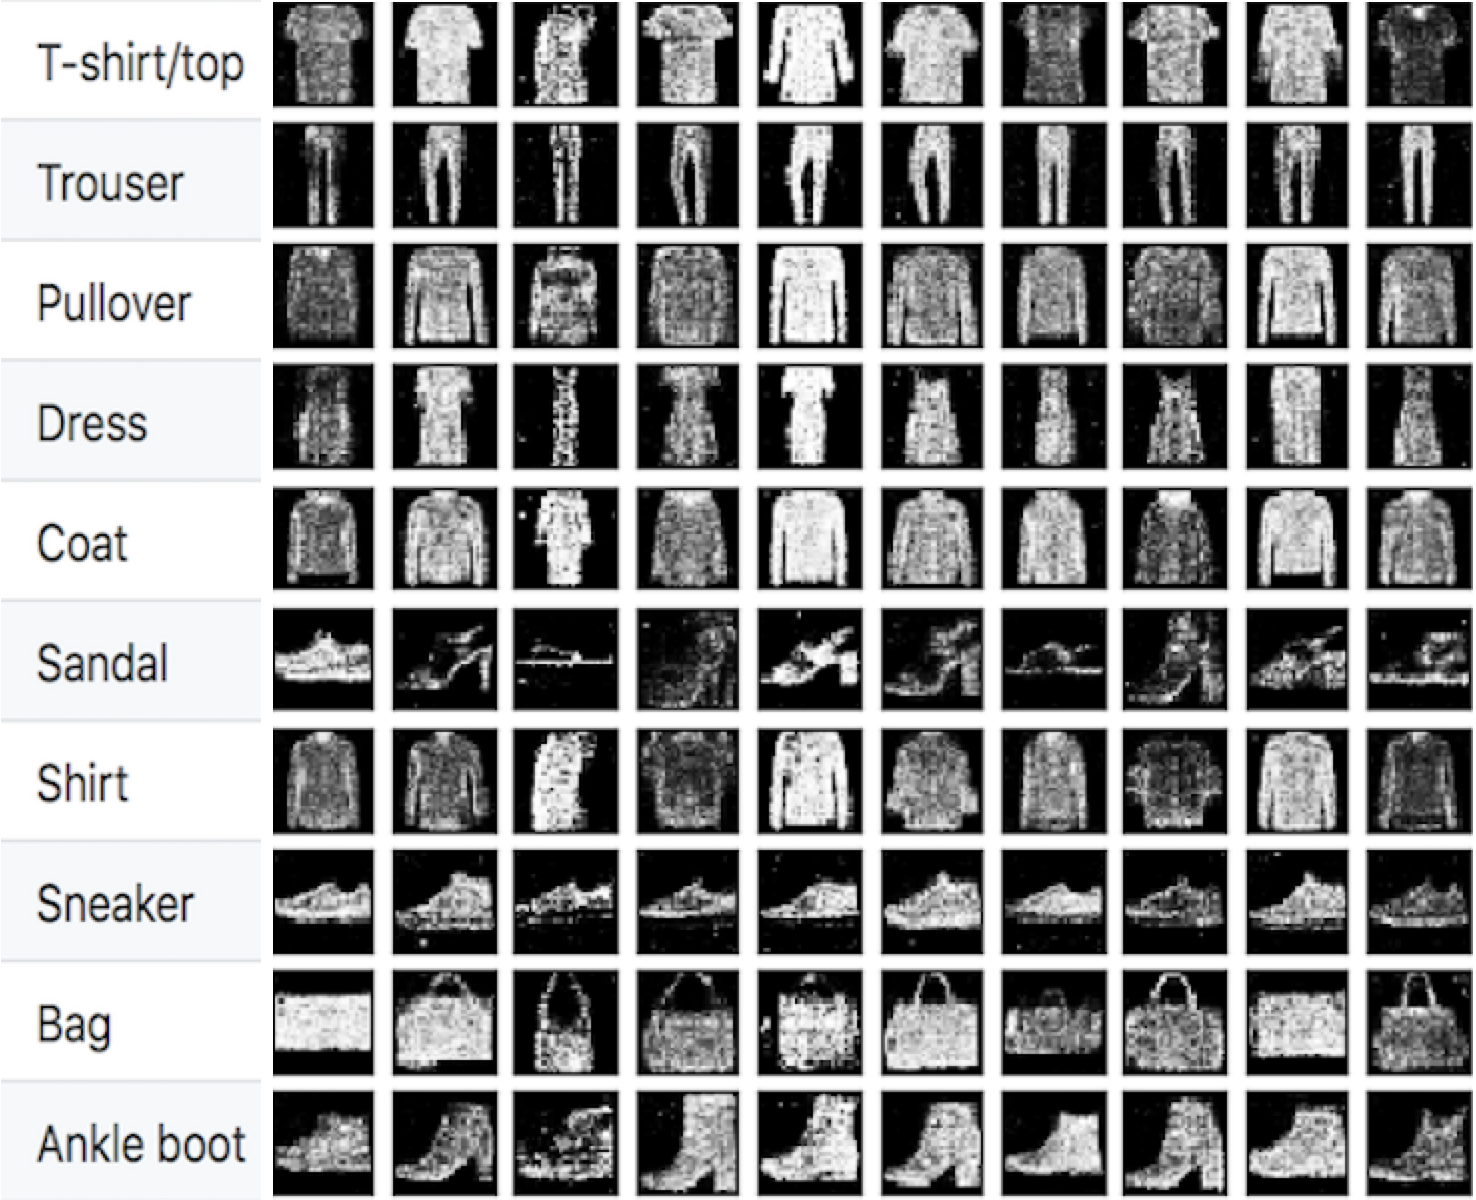
\includegraphics[width=0.8\linewidth]{label_epoch500.png}
\captionof{figure}{\color{Green} 500次迭代训练结果}
\label{500epoch}
\end{center}\vspace{1cm}

 之后,我们对渐进式增长生成对抗网络\supercite{DBLP:journals/corr/abs-1710-10196}文章的源码进行修改使其适应FashionMNIST的数据格式,之后使用该程序进行训练,得到生成结果,与我们的结果对比如图\ref{compare}。
\begin{center}\vspace{1cm}
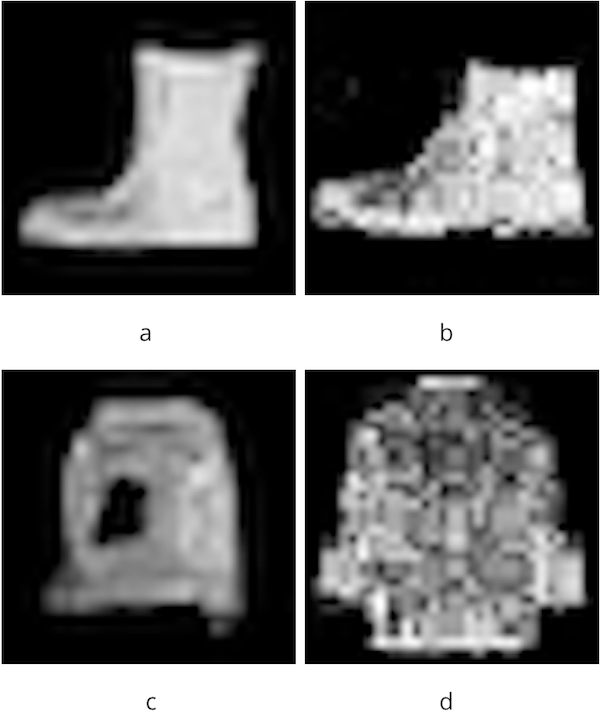
\includegraphics[width=0.5\linewidth]{compare.png}
\captionof{figure}{\color{Green} a, c 为使用PGGAN生成图片, b, d 为使用CGAN生成图片}
\label{compare}
\end{center}\vspace{1cm}

  为了验证我们的方式可以有效地避免图像识别软件对图片的分类识别,我们使用开源的图像识别程序对我们的图片和MNIST中的图片进行训练后进行识别,对两种情况下的准确率进行测试比较,识别准确率结果如图\ref{准确率比较}。可以看出,我们的图像有着很好的优势,在一定程度上干扰了图像识别程序对图像的识别的准确率。由于在我们的实验中使用的是单一的图片进行识别,因此图像识别程序经过一定的训练之后仍然可以实现较高的识别准确率,但是如果将这种方式应用到实际工业中,通过对几张图片进行组合之后构成的图片应该会有更低的准确率,从而实现我们改善图形验证码的目标。

\begin{center}\vspace{1cm}
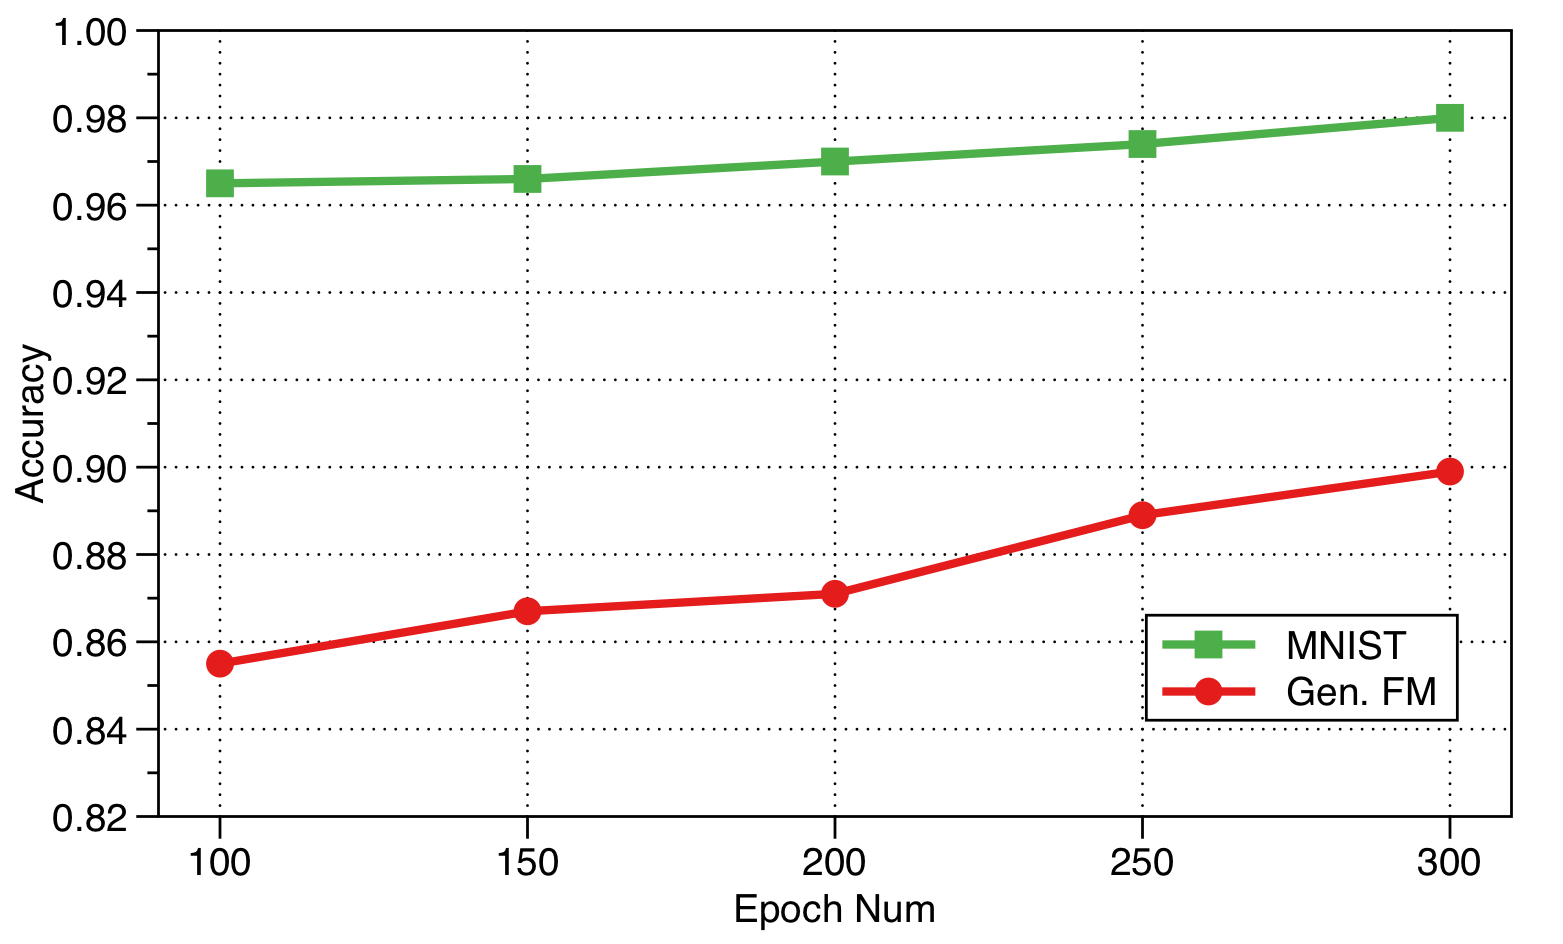
\includegraphics[width=0.8\linewidth]{Experiments.png}
\captionof{figure}{准确率比较}
\label{准确率比较}
\end{center}\vspace{1cm}


\section*{Conclusions}

  通过对两种生成方式生成的图片的细节比较,我们得到以下结论:
\begin{enumerate}
	\item PGGAN\supercite{DBLP:journals/corr/abs-1710-10196}使用从低分辨率图片开始训练的思路,因此对物品轮廓的描述十分清晰,但由于PGGAN设计针对高分辨率图片生成,因此在$28 \times 28$情况下对细节的描述并没有突出优势。
	\item 我们设计的模型利用实际图片进行训练,噪音较为严重,但是我们的结果具有准确的标签以及较好的细节处理。
	\item 因此在我们生成验证码的情形下,我们的模型在结果足够清晰的同时具有实现简单,训练速度较快,生成图片具有明确分类的优势。
	\item 通过实验验证,对应相同的图像识别程序,我们的图片可以有效降低识别的准确率。
\end{enumerate}

\section*{Forthcoming Research}

  从实验结果可以看出,我们的模型生成的图片噪点较多,轮廓不够清晰,根据PGGAN生成图片的优点,我们考虑可以将渐进增长的训练思路引入我们设计的模型。在我们设计的半监督模型下,从低分辨率开始对数据集进行训练,生成质量更高,更易辨别的验证码图片。同时,我们的图片生成模型并不局限于FashionMNIST数据集,也可以推广到更为复杂的数据集上,从而进一步改善生成图片的质量,使其更适用于验证码环境中。

\printbibliography[title={References}]
\newpage

\section* {Personal Summary}
  在人工智能导论这门课的学习过程中,我们学习了一些经典的人工智能的算法并在课程作业中进行了实践,加深了我们对课堂上学习到的知识的掌握。在大作业的完成中,我们可以开放地进行选题,尝试一些十分新颖的人工智能方面的算法,对这些算法的特性以及实现进行学习并完成自己的项目。同时,最后展示的环节采取了和以往的计算机辅修课程不相同的POSTER展示的方式,让我们可以按照自己的兴趣对同学实现的算法进行学习与讨论,让我们认识到人工智能的方法在许多方面的应用以及实现方式,比以往的课堂ORAL汇报的方式带来更大的收获。同时,采用小组共同完成一个大作业的方式不但减轻了我们的负担,还允许我们按照自己的兴趣对一个题目中的不同方面进行深入探究。这一系列较为灵活的教学方式给我们带来的很大的收获。

  最后,十分感谢老师和助教耐心的回答我们的问题以及十分认真的指导。


\section*{Distribution of Work}
\begin{enumerate}
	\item 张知行:主要负责了模型的设计、代码的编写以及实验的方案设计。
	\item 钟昊东:主要负责了模型的参数调整以及模型的训练和POSTER展示。
	\item 朱文轩:主要负责了模型对比方案的文献查找与研究。
\end{enumerate}

\end{document}




















